\chapter{Modelo \textit{Bulk Synchronous Parallel}}

O \textit{Bulk Synchronous Parallel}(BSP) é um modelo de programação que 
surgiu para que se possa fazer processamento aproveitando-se recursos 
computacionais existentes utilizando técnicas de computação concorrente.

\section{Descrição do Modelo}

A base do modelo de programação BSP consiste no seguinte:
\begin{itemize} 
 \item Componentes de processamento.
 \item Comunicação entre as entidades envolvidas no processamento.
 \item Sincronização das entidades que estão a processar.
\end{itemize}

As componentes de processamento, no BSP, estão fortemente ligadas à ideia de 
processo e de processadores lógicos. Contudo, em plataformas que se baseiam no 
modelo BSP e que estão construídas de modo a funcionarem em ambientes 
distribuídos o termo componentes de processamento vai para além dos 
processadores lógicos. Normalmente, em plataformas distribuídas, entende-se por 
componentes de processamento os vários \textit{nodes} e para cada \textit{node} 
os seus respetivos processadores lógicos. Desta forma, as plataformas 
distribuídas podem se aproveitar ao máximo da paralelização em cada 
\textit{node} e da distribuição de trabalho por \textit{node}.

\begin{figure}[H]
 \caption{Modelo BSP}
 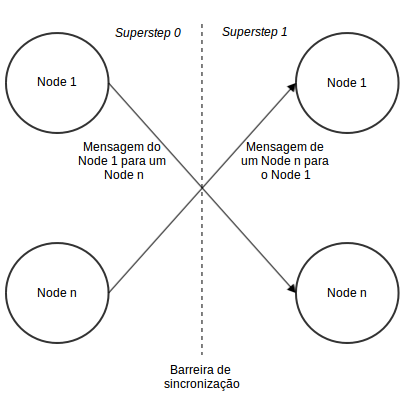
\includegraphics{bspmodel.png}
 \label{fig:bspmodel}
\end{figure}

Seguindo este modelo é possível descrever algoritmos distribuídos de forma 
progressiva, tendo em consideração o possível paralelismo da solução, devido ao 
mecanismo de comunicação e de sincronização. A sincronização das entidades é  
feita entre as diversas iterações, denominadas no modelo por 
\textit{supersteps}, o que permite a troca de mensagens entre as componentes de 
processamento de uma iteração para a seguinte como se pode ver na Figura 
\ref{fig:bspmodel}.

Num ambiente distribuído deve se ter em conta que a comunicação é normalmente 
feita através da rede, salvo exceções em que as o processamento esteja a ser 
feito no mesmo \textit{node}.

\import{"../hama-giraph comparison/"}{"HVSG"}